\section{看见}

\vspace{10pt}

{\centering\subsection*{客厅的书墙}}

\addcontentsline{toc}{subsection}{客厅的书墙}

\renewcommand{\leftmark}{客厅的书墙}

\begin{figure}[htbp]

\centering

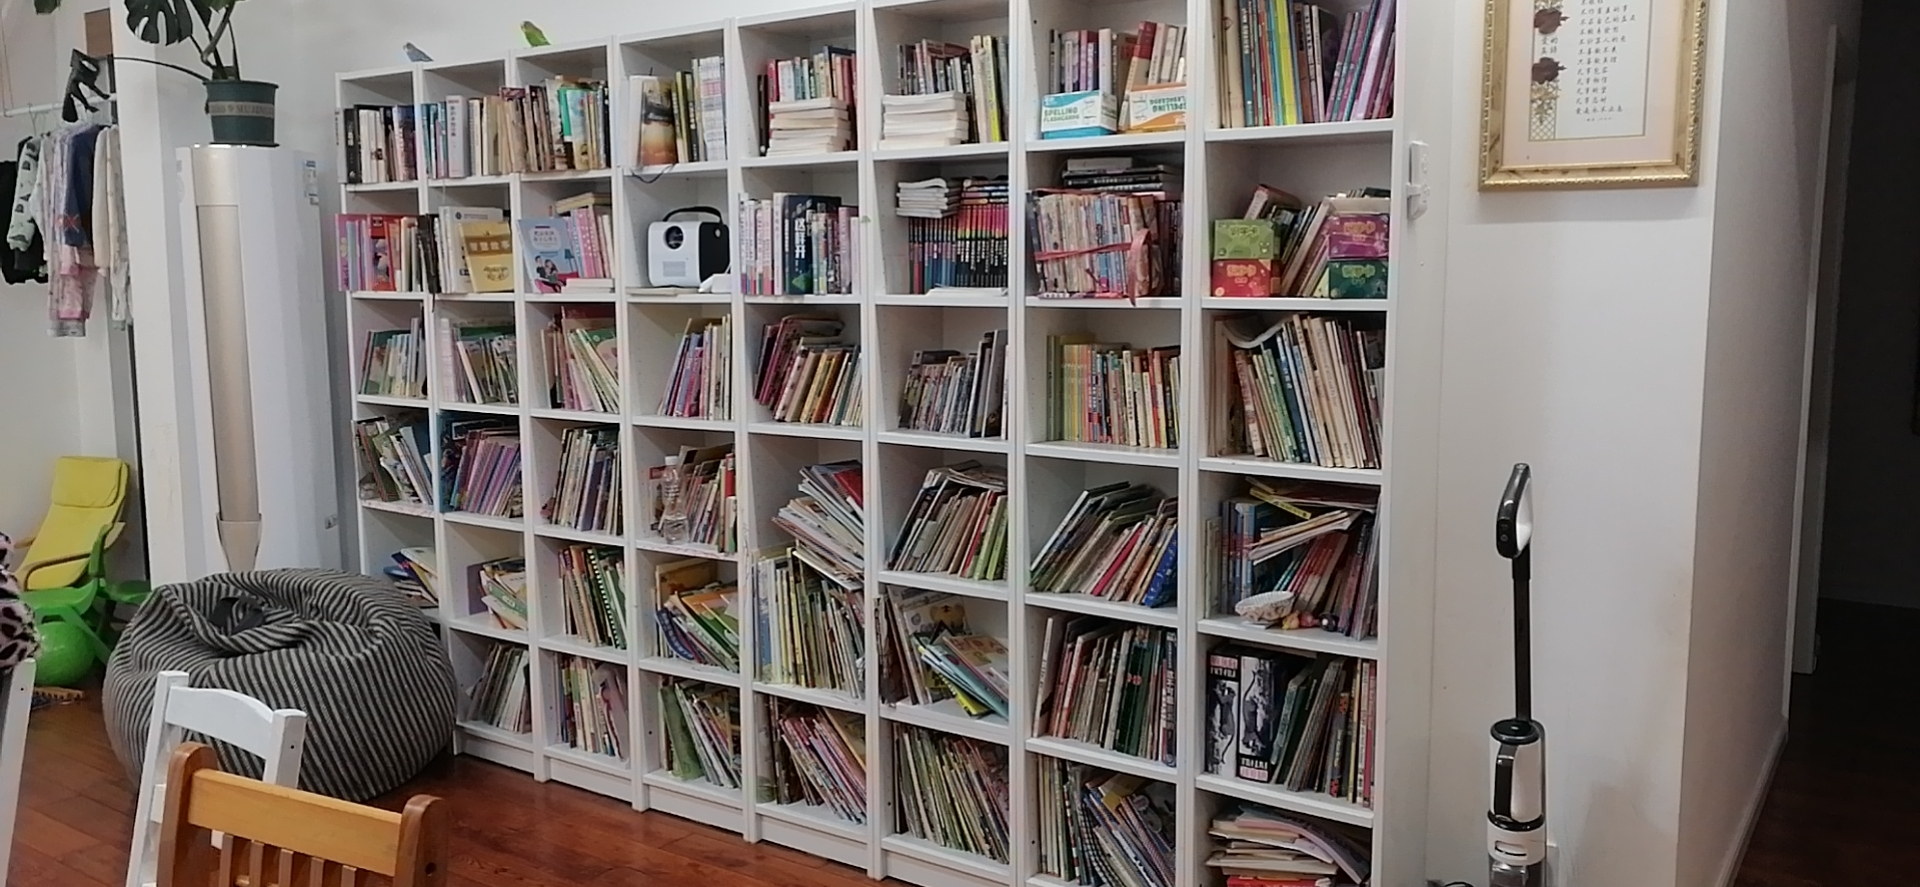
\includegraphics[width = .5\textwidth]{./ch/zzg.jpg}

\end{figure}



2014年的时候,听到柏墩小学校友要发起在桂花建立图书馆,很是有感触,自己有想过,有规划过,然而却没有实施,看到校友们在一个小镇开启了图书馆,很是开心,有幸可以参与进来,感恩能够有机会一起为图书馆做些事情。


自2012年回国后,回到家乡,曾去过小学和中学母校,校园已经有了很大的变化。然而,整个镇都没有什么可以借阅书的地方。在上海读高中,学校里有很好的图书馆,几乎每周都会去借阅书。在国外读书,几乎每个小镇上都有藏书不少的图书馆,还经常带着住家的孩子们去现场看书,借阅。也正是因为这个原因,我也很喜欢看书,一旦有好书,还会多购买些,赠与好友。


“读万卷书不如行万里路”,自己去过不同的地方,也可以阅读到不同的书,然而在老家的很多孩子们,还没有多少机会去触碰到课外书籍,更不用说“读万卷书”。从那时开始便有意识的囤积一些适合中小学学生看的书,心想以后可以建立个“图书馆”。听说桂花图书馆的建立,很是欣喜,捐出了一些囤积的书籍,有幸能够和原始团队成员沟通图书馆的管理及长期规划。


现在图书馆走了这么多年,非常不易,感恩一直在为着桂花图书馆付出的每一个人,是你们给孩子们开启了一扇通往“知识的海洋”的道路,让孩子有机会去“读万卷书”,让孩子接触到阅读。看到孩子们在图书馆畅游书的世界,满是欢喜。看到孩子的文集,可比我当初的文采好很多,也可以看出孩子的“作文”来自其他书籍的引用。同时也是很欣慰,后浪厉害了。


随着社会经济的发展,更多注重到阅读,几乎很多村委会有图书室。桂花镇柏墩社区图书馆已建立好,不管是孩子还是大人,接触到书的机会越来越多。然而随着科技的进步,看手机的越来越多,书本阅读的人越来越少,但还是鼓励我们要继续书本阅读,好书可以收藏,说不定哪一天想起来还可以再用;好书可以分享,说不定正好帮助到其他人;好书可以共享,说不定成为了其他人的榜样。


现在的社会整体都比较浮躁,很难静下心来好好拾起书本阅读,但也不是不可能。从我做起,营造一个阅读的环境,客厅一面墙的书,孩子的房间里也有他们各自翻阅最多的书,办公室也有和工作有关的书。也喜欢关注并购买最新科技,管理,教育等方面的书,觉得好的话,会购买送给朋友。倡议作为家长们,可以多拾起书来阅读,给孩子做楷模,一起阅读。孩子们,阅读可以开阔我们眼界,畅游在知识的海洋里。










\vspace{10pt}


祝振刚

桂花图书馆 名誉理事

2022年1月24日
                



\vspace{10pt}

\hline

%\clearpage


\vspace{10pt}

{\centering\subsection*{社区的“幸福之家”}}

\addcontentsline{toc}{subsection}{社区的“幸福之家”}

\renewcommand{\leftmark}{社区的“幸福之家”}

\begin{figure}[htbp]

\centering

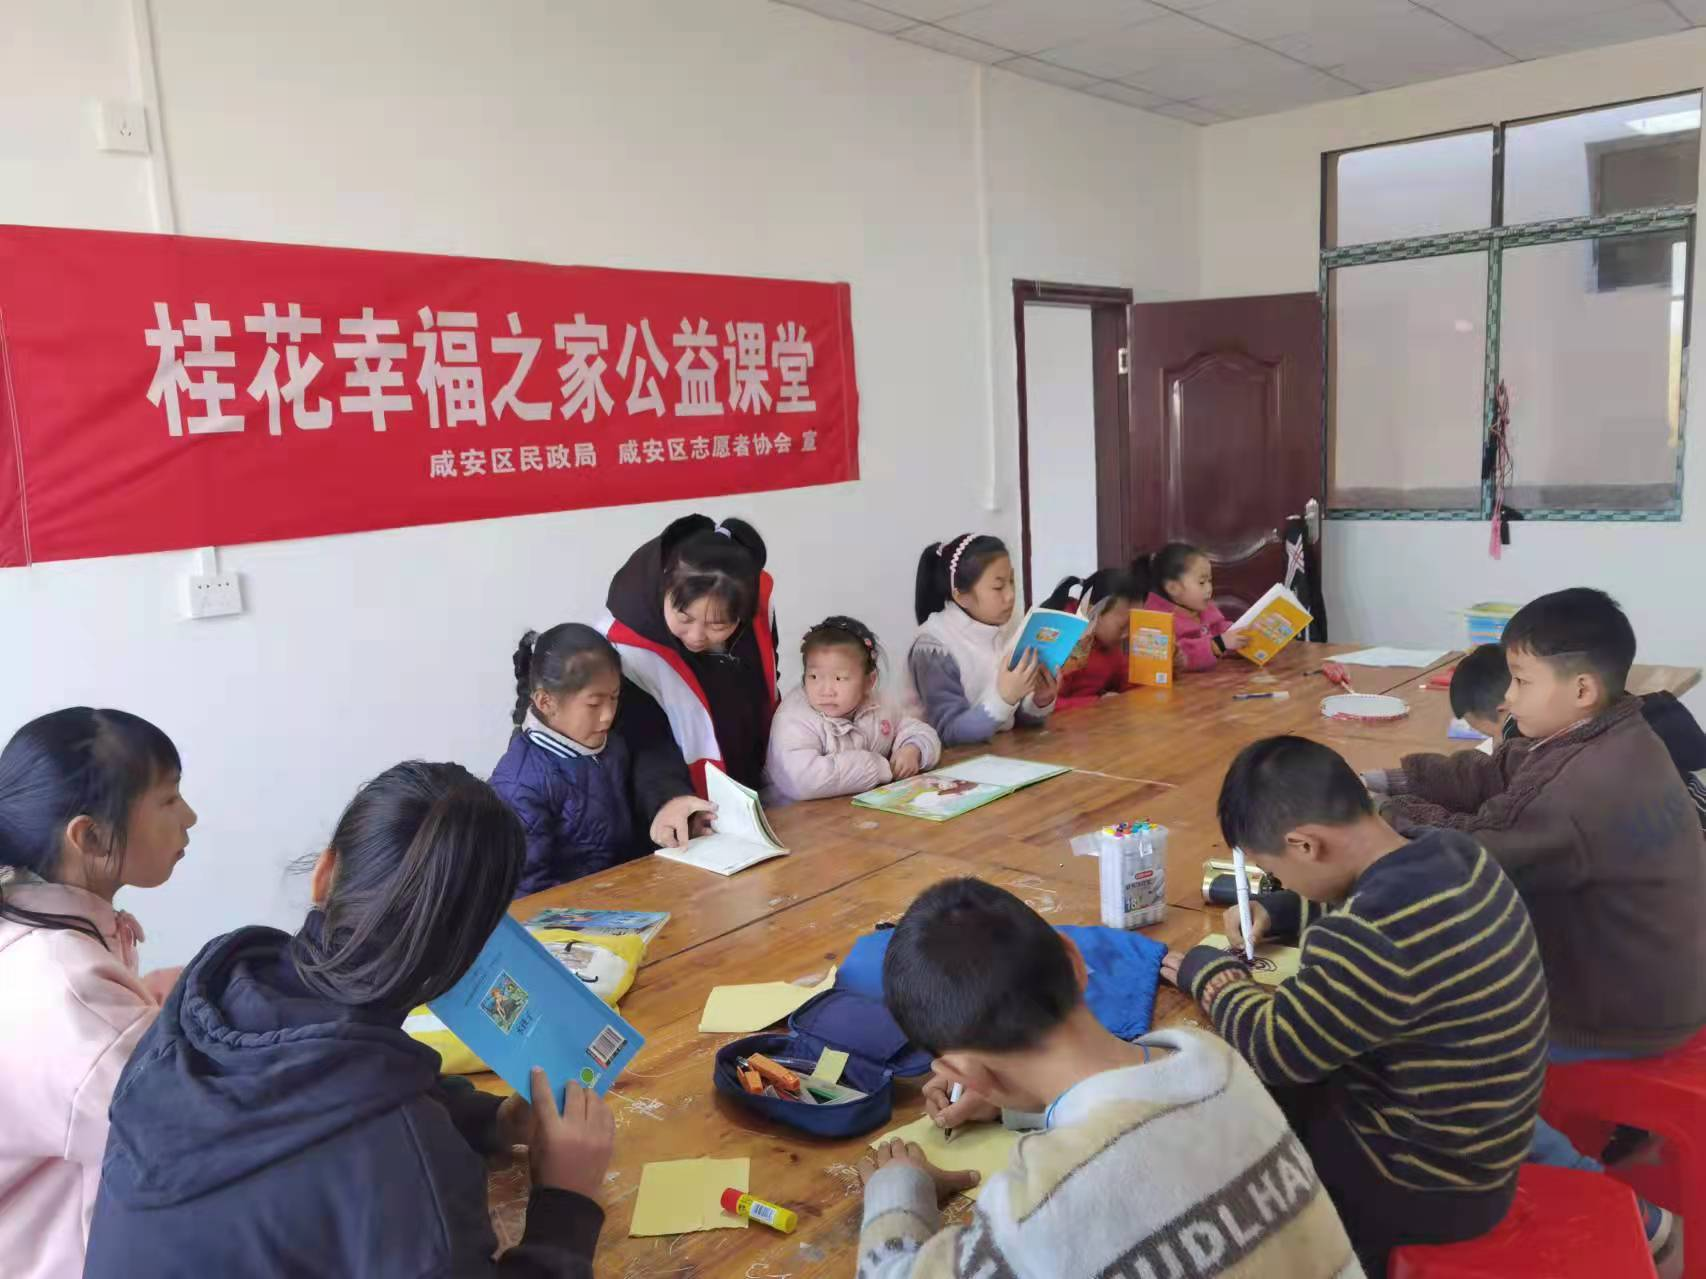
\includegraphics[width = .5\textwidth]{./ch/yjp1.jpg}

\end{figure}

桂花镇柏墩社区图书馆是在咸宁市桂花镇政府的工作指导下,创建社区志愿者文明实践站而打造的居家养老项目中的一个功能室。

社区图书馆公益项目目前的建设属于刚起步状态,立足于服务更多的社区居民,服务孤寡老人、困境老人、留守儿童、困境儿童、困境妇女。社区图书馆有着一个长远的意义,从公益服务的角度出发,它是一个服务社区居民的功能室。

受咸安区志愿者协会的支持,我是桂花镇柏墩社区服务留守儿童的公益课堂“幸福之家”的负责人。这个“幸福之家”这学期刚入驻,主要是服务更多的困境儿童、留守儿童,解决他们课后无人陪伴、无人辅导的问题。

\begin{figure}[htbp]

\centering

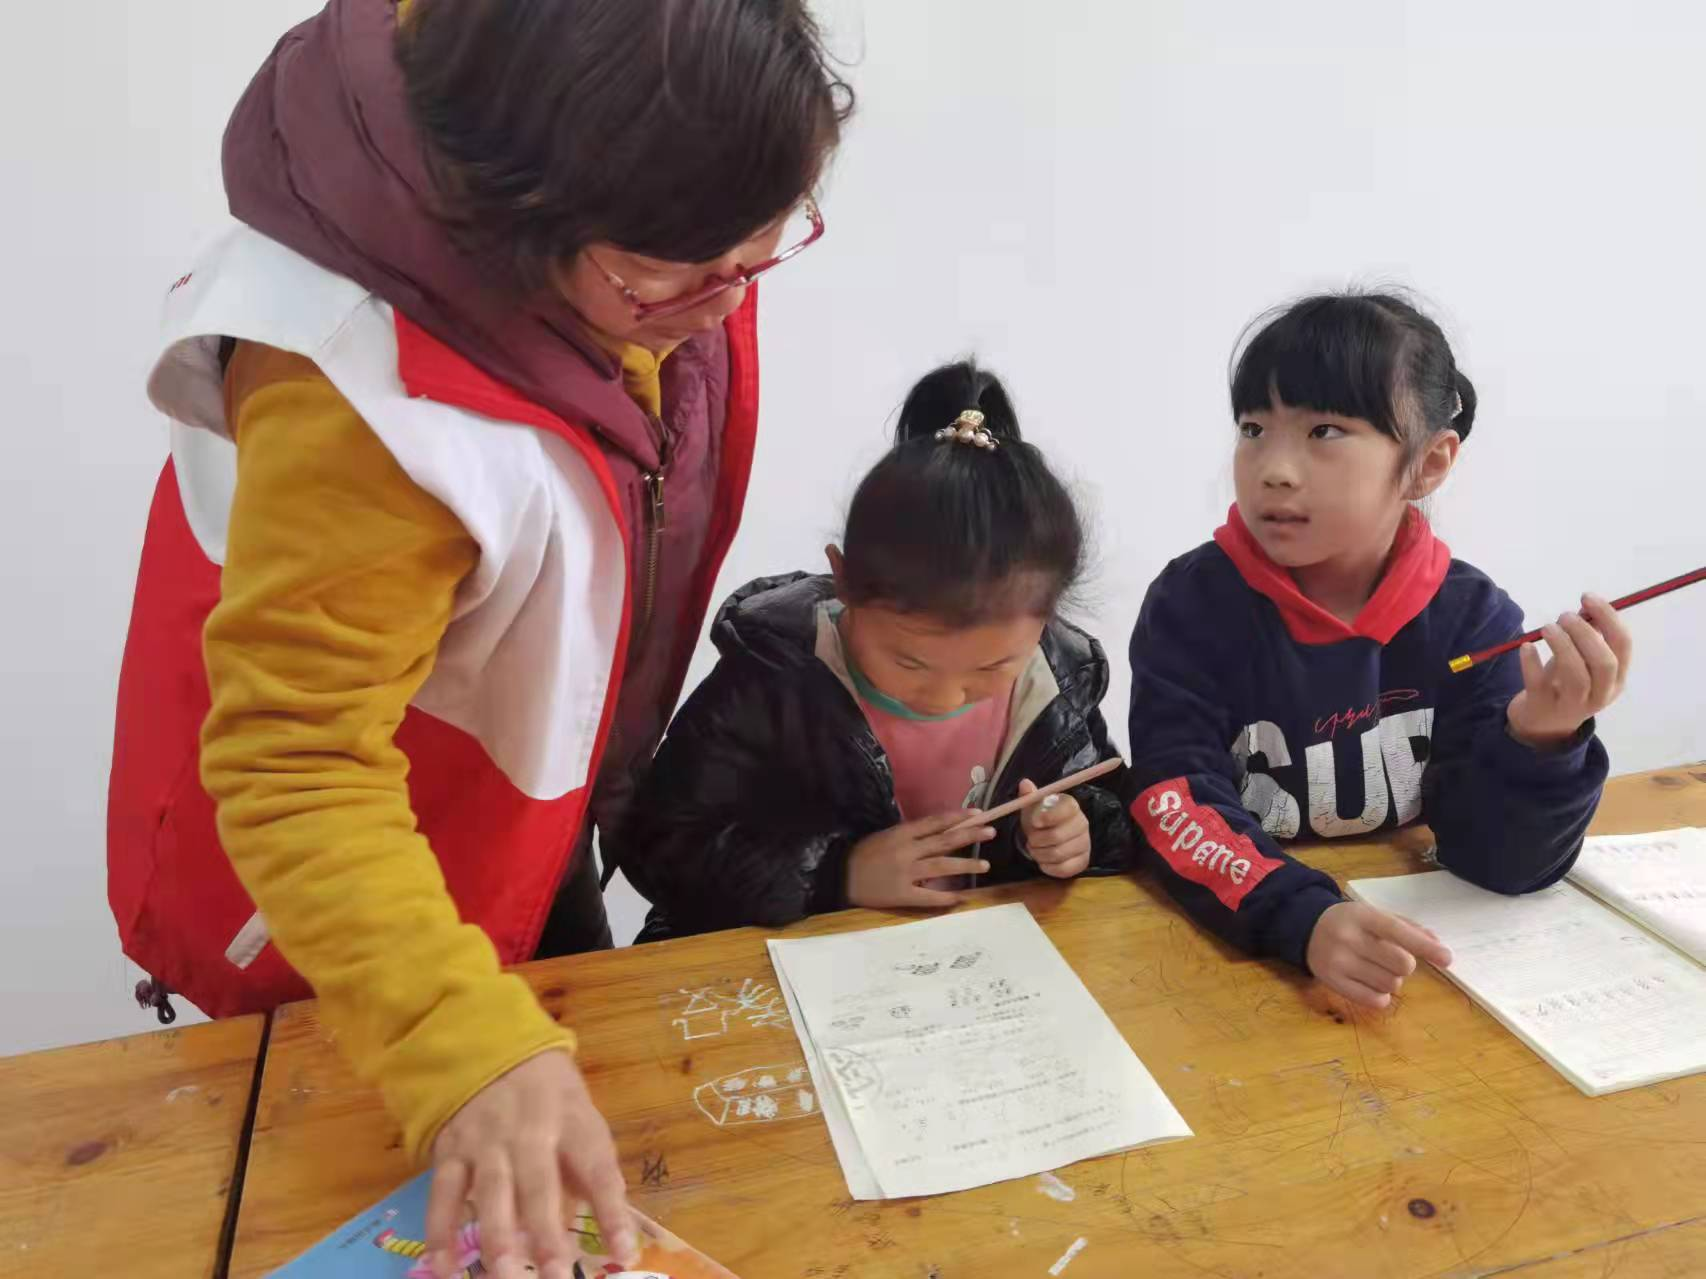
\includegraphics[width = .5\textwidth]{./ch/yjp2.jpg}

\end{figure}
    
社区志愿者文明实践站是在打造咸宁市全国文明城市一个大的城市发展的前提条件下成立的一个实践站,也是桂花镇打造的特色项目。这个实践站设立在柏墩社区服务中心内。文明实践站和居家养老虽然是分开的两个项目,但是这两个项目又是相互作用相互依存的。根据规划,整合柏墩社区的实践站和居家养老的工作资源,把居家养老活动场地进行扩建,打造成柏墩社区的一个特色项目。目前,由镇政府出资,社区管理,将桂花镇老政府办公地全面进行了改造,投资了一百多万进行了翻新修建,扩建了一些功能室。

\begin{figure}[htbp]

\centering

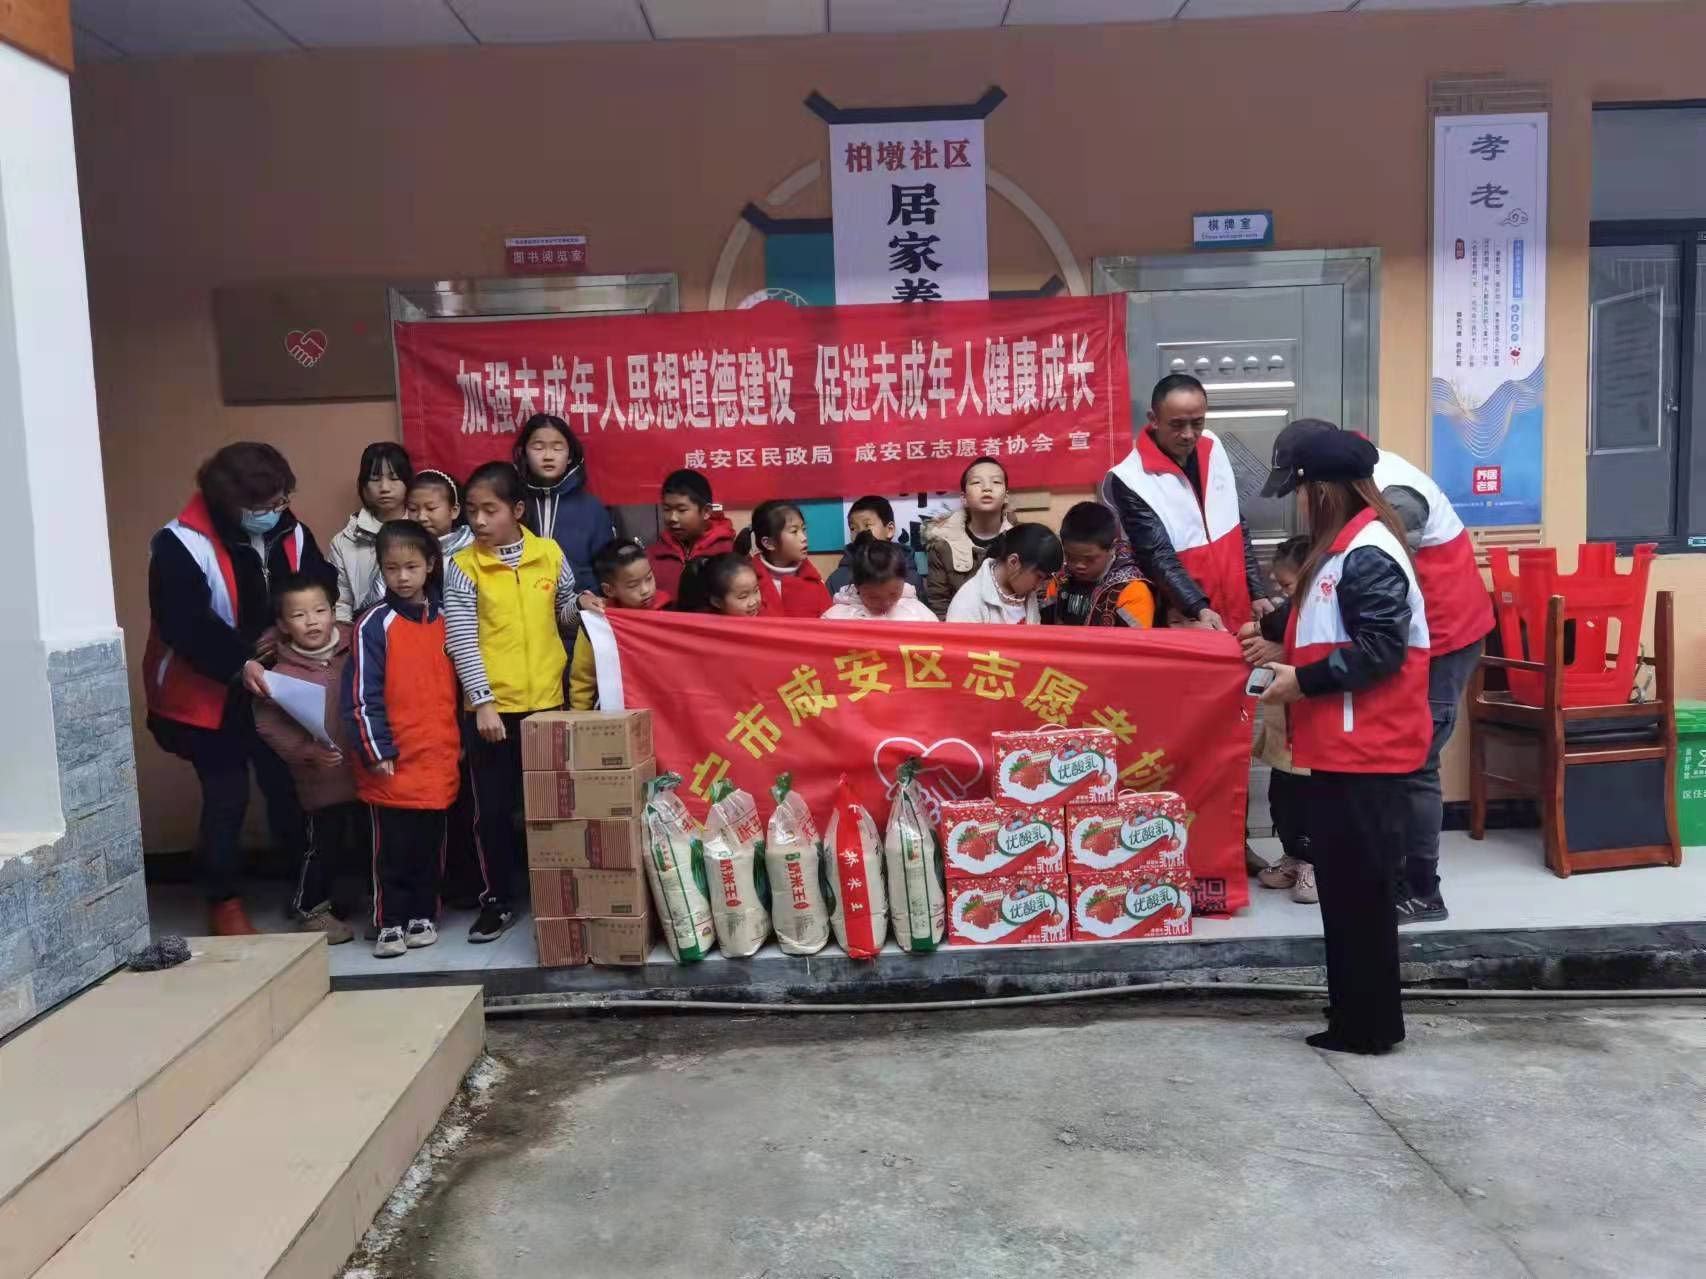
\includegraphics[width = .5\textwidth]{./ch/yjp3.jpg}

\end{figure}

就目前的现状,柏墩社区除了现聘人员之外,会通过镇政府招聘图书管理员以及其他项目的管理员,还会成立柏墩社区的志愿者服务队。
      
其次,将来老政府会改造成居家养老活动中心。目前里面居住的大多数是困境老人、租房陪读的家长与留守儿童等需要帮助的群体。改造后将改善这些群体的居住环境。

最后,改造后的活动场地环境优美。它包括了棋牌室、健身房,还有文化活动室等,功能比较齐全。但目前缺的是资源,比方说图书的资源。对于这个图书资源,可以通过政府的途径去采购,也可以通过社会爱心人士捐赠。

我觉得这是一个很好的机会,帮助社区居民获得更多的公益服务。







\vspace{10pt}


易金平

社区公益课堂“幸福之家”负责人

柏墩中心小学 前副校长

2022年1月12日
                



\vspace{10pt}

\hline
%\clearpage


\vspace{10pt}

{\centering\subsection*{疫情和双减下的阅读}}

\addcontentsline{toc}{subsection}{疫情和双减下的阅读}

\renewcommand{\leftmark}{疫情和双减下的阅读}

\begin{figure}[htbp]

\centering

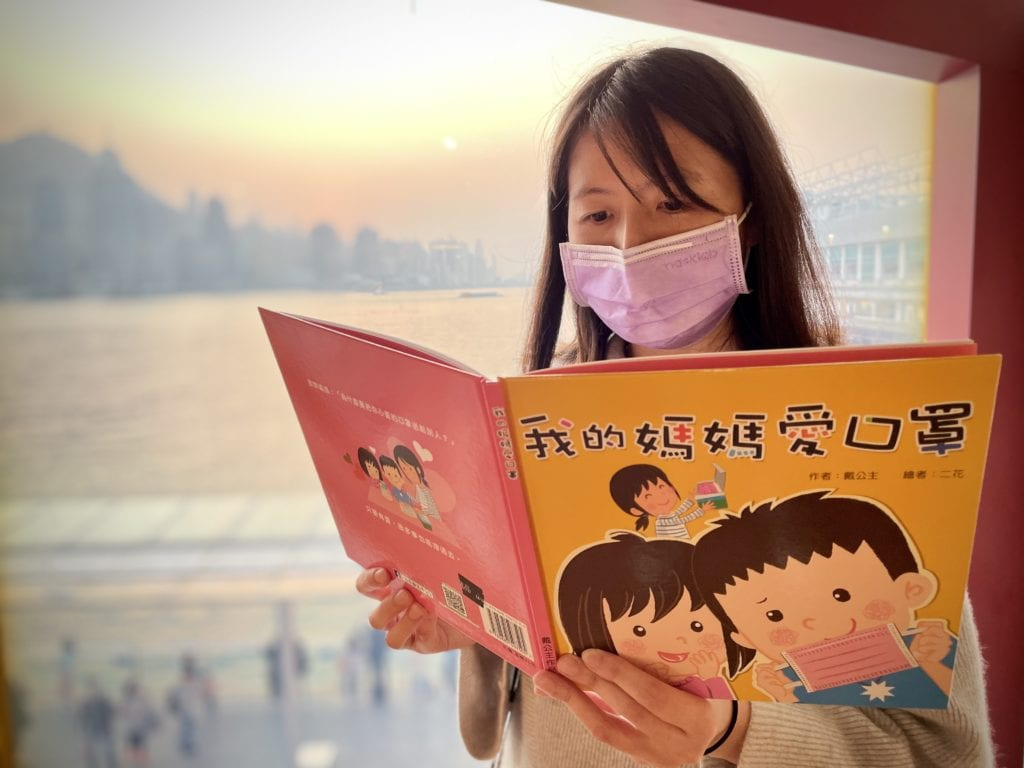
\includegraphics[width = .5\textwidth]{./ch/zj.jpg}

\end{figure}

白驹过隙,时光荏苒,很难想象,我们已经与百年一遇的新冠疫情同渡两年了。笔者去年经历了诸多悲欢离合,但总因人类难以共情而不相通,是以无多言必要。多有感慨的是:人,既脆弱,又坚强;遗忘是人类的本性,不管是情感保护机制的作用还是出于共同体进化维稳的需要。

言归正传,桂花图书馆存世已七年又八个月,到后期出于成本效果及人力财力投入状况之考虑,本已在最低限度运营。疫情第一年,上半年学校暂封,学生线上学习,无奈随之闭馆,下半年乃集体借阅。第二年上半年续之,下半年突遇双减叠加午托晚托之政策,学生在校期间缺乏借书时间,图书馆乃丧失其作用空间。经过近两个月试运行,效果难彰,是以暂停馆长馆务运行,而交予学校直接管理,以班级为单位借阅。

2022年计划新增为新成立之柏墩社区服务中心进行图书捐赠,待议定而后行之,后期亦可能携手本市志愿者协会于社区开展阅读相关活动。

漫漫公益路,如此草根之活动,坚持至今,纷争有之,焦虑有之,妥协有之,疲累失望有之,感动感恩有之,于丰沛情感不无裨补。然余不得不叹息可谓徒耗心血,寄希望于带来微小之改变,初心难改,然百年树人,效果难彰。

路在何方否?支持、参与图书馆事务的各位同仁,付出了,奉献了,也收获了。得之我幸,失之我命,奋斗不息。唯有不忘初心,方得始终。往后的日子里,唯有踔厉奋发,笃行不怠,方能不负所有支持关注图书馆的朋友的期待。
        








\vspace{10pt}


张锦

桂花图书馆 理事长

2022年1月23日
                



\vspace{10pt}

\hline
%\clearpage





\vspace{10pt}

{\centering\subsection*{阅读世界与写作人生}}

\addcontentsline{toc}{subsection}{阅读世界与  写作人生}

\renewcommand{\leftmark}{阅读世界与  写作人生}

\begin{figure}[htbp]

\centering

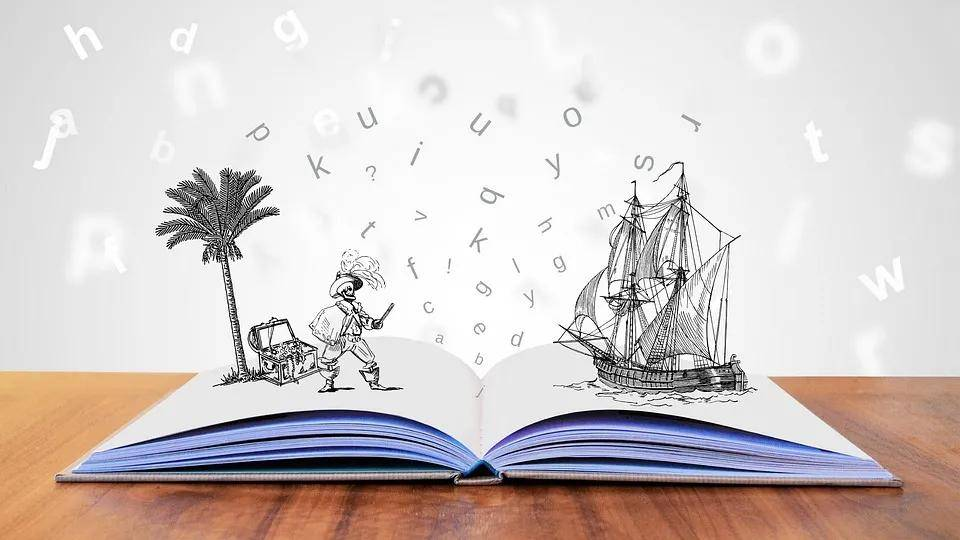
\includegraphics[width = .5\textwidth]{./ch/yhj.jpeg}

\end{figure}



 
听闻图书馆今年又出了一本作文集,我的内心是激动的,与前一本的激动不尽相同,这一次更多了对孩子们坚持写作,坚持阅读精神的感动。

在这个信息爆照的年代,孩子们能坚持在一片净土中,徜徉于书海,并用自己笔写自己的心,这真的是一件让人开心且为之自豪的事。

在三到六年级的孩子的作文里,我感受到了浓浓的童真童趣,一个个跳动的字符,一句句灵动的话语,都让我和孩子们有次心灵的对话。
阅读、写作是孩子们用心和世界交流的过程,在这个过程中,会丰富孩子们的精神世界,会让孩子们真正做自己的主人。

“小荷才露尖尖角,早有蜻蜓立上头”,希望我们的孩子们,能继续坚持阅读和写作,继续用笔抒发自己的情感,和世界对话。愿更多的孩子们能爱上阅读,爱上写作。
   

 


\vspace{10pt}

 于鸿锦

柏墩中心小学文学社社长

2022年1月15日
                



\vspace{10pt}

\hline
%\clearpage


\vspace{10pt}

{\centering\subsection*{我当馆长这一年}}

\addcontentsline{toc}{subsection}{我当馆长这一年}

\renewcommand{\leftmark}{我当馆长这一年}

\begin{figure}[htbp]

\centering

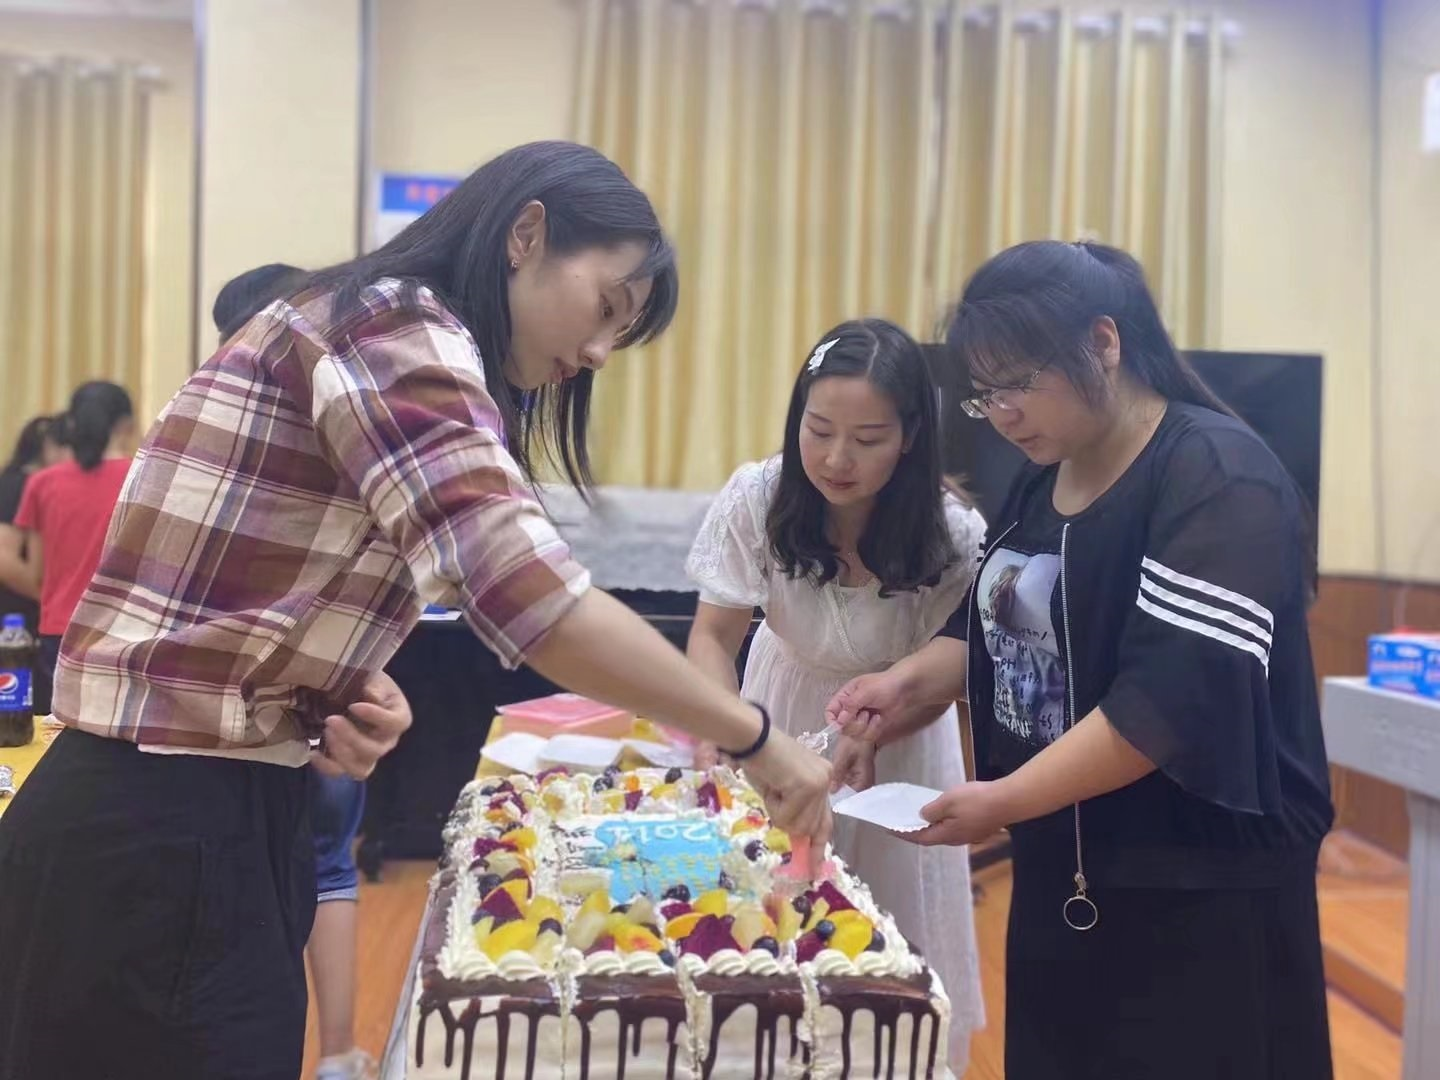
\includegraphics[width = .5\textwidth]{./ch/mjq.jpg}

\end{figure}



一个偶然的机会,我加入了桂花图书馆的大家庭。从陌生到熟悉,我不断努力学习着,逐渐的爱上了图书馆这份平凡的工作。

图书馆的工作看似简单也就“借借还还”,其实也是一项复杂、细致而繁琐的艰苦工作,需要有耐心细致周到的服务态度。一开始我也有点打退堂鼓,但是在看到孩子们求知若渴的眼神时,我还是慢慢地坚持下来了。当然这也要感谢图书馆的执行团队和我们可爱的孩子们。因为有图书馆执行团队的协助让我更快地适应工作。因为有孩子们让我每天置身于孩子们纯真的笑脸之中,让我听到了充满理想的声音,让我感受到了青春的气息。

每当在编辑孩子们的作文时。我看到这些朴素稚嫩而又鲜活的文字,内心的尘垢会被慢慢地拭去,内心充盈着感动。被文字牵引着,被意心的真诚完美善良感动。

只要有纯真的童心相伴,你就能够用手中的笔,写出让人眼睛发光的文句。愿更多的孩子们能在书籍的海洋里体会语言的魅力,感受到阅读的快乐!
 


\vspace{10pt}

 莫静琴


桂花图书馆 馆长

2022年1月15日
                



\vspace{10pt}

\hline



\clearpage

             
